%!TEXroot = ../thesis-main.tex

\chapter{Scenario di riferimento}

% Introduzione alle motivazioni che spingolo 'utilizzo di un software come Alchemist

\subsection{Un software complesso: Alchemist}\label{sec:alchemist}
Alchemist\cite{Pianini_2013} è un framework di simulazione open-source sviluppato dall'Università di Bologna, progettato per modellare elementi di programmazione pervasiva. Per comprendere l'ambito del progetto è necessario introdurre il concetto di simulazione in ambito scientifico. Per simulazione si intende un modello della realtà, costruito secondo le regole di un analista, sviluppato per consentire la valutazione dello svolgersi di una serie di eventi in un ambiente definito. Lo svolgimento di una simulazione avviene all'interno di un arco di tempo discreto suddiviso in unità di tempo predefinite conosciute come \textit{step}. Alchemist, consente di creare, osservare ed analizzare simulazioni atte a modellare interazioni tra agenti autonomi in ambienti dinamici: ossia scenari di \textit{aggregate} e \textit{nature-inspired computing}. Una rappresentazione del meta-modello, ossia le entità e relazioni configurabili, è raffigurata nella \cref{fig:alchemist-metamodel}.

\imagesource{figures/alchemist-metamodel.pdf}{https://alchemistsimulator.github.io/explanation/metamodel/}{Il meta-modello di Alchemist}{.9}{alchemist-metamodel}

\paragraph{Architettura} % Ulteriori spiegazioni magari sull'architettura già presente di una pipeline di continuouos integration
Il framework è realizzato mediante linguaggi JVM-based, più precisamente Java e Kotlin, utilizzando una struttura modulare ed estendibile. Il simulatore, come già citato, è un progetto open-source, ossia distribuito sotto termini di una licenza aperta. Questa permette a tutti di osservare il codice sorgente e di contribuire allo sviluppo del progetto, coordinato da un personale responsabile del suo avanzamento. La natura open-source del progetto apre le porte a modalità di sviluppo del codice differenti rispetto a team di dimensioni ridotte. In un progetto aperto, gli utenti che contribuiscono allo sviluppo sono potenzialmente infiniti, ragion per cui l'automazione risulta determinante per mantenere un processo ordinato e controllato di integrazione e rilascio del software.

\section{Tecnologie}\label{sec:technologies}

\subsection{Gradle}

Mentre in passato la produzione di artefatti (documentazione, pacchetti, eseguibili) era delegata a script costruiti dallo sviluppatore, in un progetto di grandi dimensioni è oggigiorno essenziale avvalersi di uno strumento di \textit{build automation}. Come l'output di un programma deterministico non cambia per uno stesso input, la produzione di artefatti deve essere consistente e riproducibile riducendo al minimo l'intervento umano. 

Gradle\footnote{https://gradle.org/} è uno dei tanti strumenti disponibili, supporta diversi linguaggi di programmazione anche se risulta popolare nell'ambiente JVM come alternativa a Maven. I \textit{task} sono l'unità minima di esecuzione e rappresentano un azione: come generare un JAR, eseguire dei test o produrre la documentazione. Mediante direttive come \textit{dependsOn} è possibile creare dipendenze tra processi: Gradle orchestra l'esecuzione dei task costruendo un grafo aciclico diretto (DAG) delle dipendenze. L'esecuzione di Gradle avviene in tre fasi distinte elencate di seguito.
\begin{enumerate}
	\item \textbf{Fase di inizializzazione}: in primo luogo Gradle crea un'istanza di Settings che organizza l'architettura del progetto. Attraverso un file, di nome ``settings.gradle", lo sviluppatore stabilisce il progetto radice e tutti gli eventuali progetti figli. 
	\item \textbf{Fase di configurazione}: successivamente tutti i file di configurazione ``build\-.\-gradle" (del progetto radice e tutti i sotto-progetti) vengono analizzati per costruire il grafo dei task.
	\item \textbf{Fase di esecuzione}: infine, Gradle esegue i task richiesti considerando le dipendenze descritte nel grafo generato nella fase precedente.
\end{enumerate}

\imagesource{figures/gradle-build-lifecycle-example.png}{https://docs.gradle.org/current/userguide/build_lifecycle.html}{Esempio di inizializzazione, configurazione ed esecuzione di una build Gradle}{1}{gradle-build-lifecycle}

Un componente chiave sono i plugin, i quali consentono di estendere le funzionalità di Gradle: aggiungere nuovi task, estendere il modello con nuovi elementi ed applicare configurazioni specifiche all'intero progetto. La presenza di diversi plugin base e creati dalla comunità rende Gradle uno strumento versatile.

\subsection{GitHub Actions}

Tramite Gradle lo sviluppatore è in grado di eseguire procedure articolate come compilazione, test e dispiegamento utilizzando un semplice comando da \ac{cli}. L'invocazione di queste procedure richiede però l'intervento umano, è quindi necessario uno strumento capace di automatizzare i processi offrendo un infrastruttura resiliente e facilmente accessibile.

GitHub Actions è una piattaforma di \ac{cicd} disponibile per i repository ospitati su GitHub, che consente la configurazione ed esecuzione di pipeline personalizzate, chiamate \textit{workflow}. Questi \textit{workflow} sono flussi di processi che consistono in un insieme di \textit{job} eseguiti sequenzialmente o parallelamente all'interno di macchine virtuali denominate \textit{runner}. I workflow (\cref{fig:github-actions-example}) sono descritti in file YAML all'interno di una cartella specifica del repository. Questi file definiscono i passaggi (\textit{step}) e le azioni (\textit{action}) che il runner deve eseguire all'interno di \textit{job}, macro-processi incaricati all'esecuzione sequenziale di step.

\imagesource{figures/overview-actions-simple.png}{https://docs.github.com/en/actions/learn-github-actions/understanding-github-actions}{Sintesi dei componenti utilizzati su GitHub Actions ed esempio di un workflow}{.9}{github-actions-example}

Uno step, come citato precedentemente, rappresenta l'unità minima di esecuzione all'interno della piattaforma Actions. Le API supportano due differenti tipologie di step: (i) le azioni, ossia componenti riutilizzabili e parametrizzabili delegati all'esecuzione di una procedura specifica e (ii) i comandi shell. Le azioni possono essere create personalmente o riutilizzate attingendo da un vasto marketplace manutenuto dalla comunità.  Ad esempio, una delle azioni più diffuse e utilizzate è ``actions/checkout" [\cite{github-actions-diffusion}], la quale clona il repository del progetto nella cartella di lavoro corrente del runner.

\subsection{Package manager}

Il \textit{package management system} è un insieme di strumenti software che gestiscono i processi di installazione, aggiornamento, configurazione e rimozione di applicativi dal sistema. Tipicamente, ogni pacchetto corrisponde ad un singolo programma o applicazione, tuttavia, esistono anche applicazioni più complesse composte da numerosi pacchetti correlati. Il sistema di gestione dei pacchetti opera attraverso tre componenti principali:

\begin{itemize}
	\item Un componente a basso livello, che si occupa principalmente dell'installazione o rimozione dei pacchetti. Ricoprono questo ruolo: \textbf{rpm} il quale gestisce gli omonimi pacchetti e dpkg relativamente alla tipologia \textbf{deb}.
	\item Un componente ad alto livello, il cui compito principale è quello di fornire un'interfaccia all'utente come: \textbf{yum} per Fedora o \textbf{apt} per Debian. Si occupa inoltre di risolvere le dipendenze e gestire le sorgenti esterne (repository).
	\item I repository, ossia archivi pubblici ospitati online dalla quale l'interfaccia ad alto livello ottiene i pacchetti ed i relativi meta-dati.
\end{itemize}

\begin{figure}[H]
	\centering
	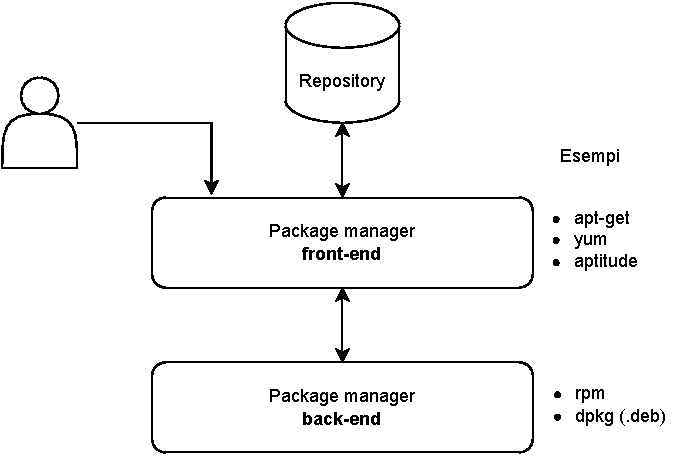
\includegraphics[width=.7\linewidth]{figures/package-managers.pdf}
	\caption{Struttura più diffusa dei sistemi di gestione di pacchetti}
	\label{fig:package-managers}
\end{figure}

L'utilizzo dei package manager fornisce diversi vantaggi nella gestione di un sistema: semplifica notevolmente il processo di aggiornamento, in quanto mediante un comando è possibile aggiornare tutti i componenti, ed allo stesso tempo, funziona da strumento di installazione capace di reperire pacchetti distribuiti in archivi online ed installarli correttamente assieme alle dipendenze richieste. 
